\documentclass[12pt]{article}
\usepackage[a4paper,margin=1in]{geometry}
\usepackage[utf8]{inputenc}
\usepackage[english]{babel}
\usepackage{graphicx}
\usepackage{csquotes}
\usepackage{setspace}
\usepackage{biblatex}
\usepackage{hyperref}

\graphicspath{{./}}
\addbibresource{bibliography.bib}

\title{A Machine Learning Approach to Building a Chess Engine}
\author{Daniel Cloutier \and Sagar Patel}
\date{\today}
\doublespacing

\begin{document}
    \begin{singlespace}
        \maketitle 
    \end{singlespace}

    \tableofcontents

    \clearpage

    \begin{abstract}
        In the current era, high volumes of data are being collected at an incredible velocity. Much of this data is embedded with valuable knowledge. \cite{main} One example of the types of data that is collected is chess data. In fact, \href{https://lichess.org/}{lichess.org}, one of many websites where chess can be played online against opponents from around the world, contains a data dump of over one and a half billion games, seventy eight million of them being played in the month of November 2020 alone \cite{lichessdb}. We intend to present an automatic learning method for chess, utilizing deep neural networks. We created our deep neural network using a combination of both unsupervised and supervised training. Employing unsupervised training, our engine pre-trains to identify and extract high-level features that exist in a dataset of chess board positions. The supervised training compares two chess positions and evaluates the board which is more favourable, from the white player's perspective. Therefore, we create a deep neural network that can understand chess without incorporating the rules of the game and using no prior manually extracted features. Instead, the system is trained from end to end on a large dataset of chess positions. The resulting deep neural network should allow for simulations that extend the possibilities of chess strategies, highly valuable to chess players at all levels.
    \end{abstract}
        
    \section{Introduction}
    The game of chess is a very popular board game and has become a well liked study for computer enthusiasts, especially in the domain of Artificial Intelligence, from the creation of Deep Blue in 1996 which defeated the world chess champion at the time, Garry Kasparov, up to modern data analysis techniques being tested on chess games as a show for it is possible uses \cite{maiachess}\cite{piece_values}\cite{alphazero}. Chess has become a good starting point for both more advanced software developers attempting to test something innovative or for newcomers trying to increase their knowledge. 

    One of the many reasons for the game's popularity is that chess data is collected at an incredibly high volume and velocity. Not only this, but the data collected is often readily available to the public. Databases such as \href{https://database.chessbase.com/}{chessbase} and \href{https://database.lichess.org/}{lichess} contain thousands, if not millions of games in a standardized notation format for chess called Portable Game Notation. This makes the game of chess a perfect starting point for new tools in Data Science to be tested.

    Another of the many domains of study that has been recently using chess as a means of improving itself is that of Machine Learning. Namely, with the advent of algorithms such as AlphaZero \cite{alphazero}, some new ideas have risen in an attempt to create algorithms that not only play chess better than humans, but even some that try and mimic human play \cite{maiachess}.

    Keeping all of this in mind, we wanted to take advantage of the very large amount of data stored by \href{https://lichess.org/}{lichess} in order to implement and perhaps try and reinvent some already existing ideas using this data that, as far as we could tell, has not been used much in recently published material.
    
    \section{Review of Research and Ideas}

    \subsection{Chess Game Categorization}

    A possibility for using this data is to attempt to categorize chess data into different groups based on some sort of requirements that we could find. For example, perhaps we could group games based on similar openings \cite{eco}, similar player ratings or perhaps try to find some different parameters to use to categorize them. One example comes by defining a distance between two games.

    One such way is defined as follows. Defining a nine dimensional space, consisting of the x-y location of a piece before it has been moved as well as after, a weight for the piece before it was moved as well as after (because of piece promotion) as well as the piece that was captured, as well as x-y locations for the piece that was captured. From here you can compare moves between games and calculate the distance between them to figure out what games are similar and what games are outliers \cite{main}. This information could be easily stored although incredibly voluminous. Every move of the game would be stored as nine seperate values. Figures \ref{fig:storing9d} and \ref{fig:piece_weights} show how storing this information could look.

    
        \begin{figure}[ht]
            \centering
            \caption{How storing the above information would look like}
            \label{fig:storing9d}
            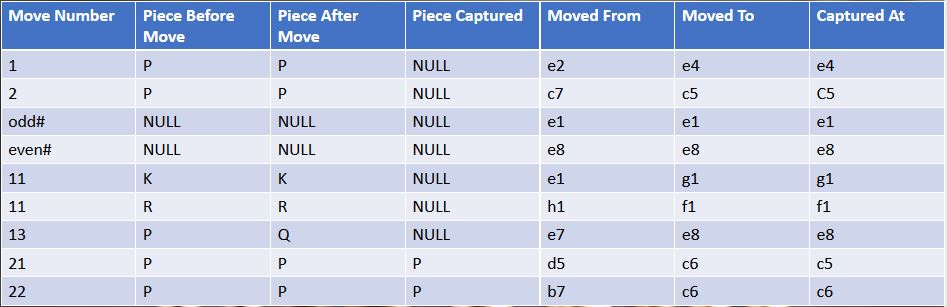
\includegraphics[width=0.9\textwidth]{9dboard.jpg}
        \end{figure}
        \begin{figure}[ht]
            \centering
            \caption{Sample weight values for pieces}
            \label{fig:piece_weights}
            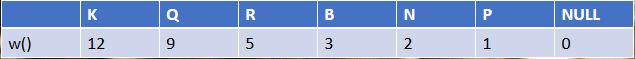
\includegraphics[width=0.7\textwidth]{sampleweights.jpg}
        \end{figure}

    From here on we can define the distance between two moves as a euclidean distance between two moves defined by this nine dimensional space. To extend this further, we can define the distance between two whole games as a sum of the distance between corresponding moves. This would be defined as 

    \begin{equation}
        dist(F, G) = \sum^{M}_{i=1} dist(F[i], G[i])
    \end{equation}

    where F[i] is the $i$-th move of game F, G[i] being the $i$-th move of game G and M is the greater of the maximum number of moves from either game \cite{main}. Appending a NULL move as necessary.

    This kind of categorization could be very useful for new and old players alike. To be able to choose a game and immediately be given results for similar games is a very powerful learning tool. There are often \href{https://www.chessstrategyonline.com/content/tutorials/basic-checkmates-smothered-mate}{patterns} that can emerge from chess positions which can likely be spotted by thorough study of similar positions or games. Also, for an advanced player, studying games that lie outside of the norm can be a good way to surprise unexpecting opponents with new ideas.

    The above is in fact a type of unsupervised machine learning. But what we can also do by using data mining techniques is create a supervised pattern matching algorithm to classify similar positions \cite{main}\cite{association}. Once again, this idea can help categorize games into buckets which can then be looked at if there are certain themes that you know of which appear in a certain group. Seeing other similar games could grant some insight into those types of positions, whether you want to learn the basics of them or want some fresh ideas to improve your play.

    \subsection{Predicting Game Results}

    Following from the previous idea, we could try to use the data in an attempt to predict the result of a game. The lichess database contains a lot of information which others might not. Based on our research, most uses of chess data was limited almost exclusively to Grandmaster games, in a specific time control, all as defined in the FIDE rulebook \cite{fiderules}. Lichess contains players of all levels, games are played in all sorts of time controls including fast one minute "bullet" games, all the way up to thirty minute slow games \cite{lichessdb}. Using all of this information, along with what was defined previously and the fact that we know the result of every game in the database, we could try and define some way to predict whether a current game of chess, given the player ratings, other similar games, time control and so on, is going to be a win for white, black or a draw.

    For example, say we could plot all games according to their similarity distance as defined above \cite{main}. However, if we were to include things like player rating, opening used, time control and so on, we could plot games on multiple dimensions. From here, by looking at games similar to an input game and looking at their results, we could make an attempt at predicting what the result of that game will be in its current state.

    There's even more than we can do still. The lichess database starting April 2017 also includes the exact clock times on every single move played. Keeping this in mind means we can improve the above idea further. Some of these could be including the current amount of time each player has, trying to improve the way we define how similar two games are or even by defining a function for determining whether a board position is winning or losing from the white player's perspective assuming best play, not unlike what modern chess computers do \cite{stockfish}. 

    Using the above information we could try and create an algorithm that would predict whether a game is winning or losing by looking at not only perfect play, but also factoring in things like time trouble and player strength. For a spectator or someone doing analysis, this could be much more insightful as to the dynamics of a position when looking at a game between two specific players instead of looking at a number which assumes best play from both sides.

    \subsection{Creating a Chess Engine}

    Moving on with this idea raises the main point for this project. Could we use all of the previous information to create an algorithm that could actually play the game of chess at a human or superhuman level. This appears to be a common theme in the field of Data Science; how to use data to improve the way we look at a certain field. We could attempt to create our own heuristics for what is important and what is not for trying to consider a certain move, however we decided on a different idea. 

    With a lot of superhuman chess engines like Komodo, Houdini and Stockfish, they have evaluation functions that are based on hard coded values for things like pieces and piece placement, as well as the stage of the game. With this in mind, we considered using something similar along with the rest of the data that we had, but try and make the piece values more accurate via some other resources like regression analysis \cite{piece_values}. This paired with the rest of our data would hopefully allow us to more easily change the difficulty of our chess engine. 

    Keeping this in mind with the rest of our information, we considered some sort of artificial intelligence that could learn on its own instead of us giving the parameters. We are not chess professionals, but there are indeed ways of getting a computer to learn, especially with large volumes of data like we have at hand \cite{mltypes_book}\cite{mlbook}. This would mean we could generate something useful despite lack of knowledge in the field. Based on our research, this theme comes up often in Data Science, especially when it comes to knowledge discovery. If we give it the parameters that determines whether a position is winning or not, for the computer to make its move, it will only reflect our own knowledge of the game. Of course, seeing as we are not expert chess players, this is not what we want. If we want to learn something new by creating this chess engine, we believed the best approach would be to let the computer use this data to learn on its own.

    \section{Problem Statement}

    Now that we know what we want to do, how exactly do we approach this problem. Surely we are not the only ones that have thought of creating a chess engine that learns on its own. This of course is indeed the case. There have been some attempts at making a self-learning chess engine, however these attempts mainly focus on learning from self-play; the computer knows the rules of chess exclusively and by playing against itself millions of times can learn on its own what wins and what does not \cite{leelachess}\cite{alphazero}. This is not necessarily what we want. We already have the data we need, it is now just a matter of getting the computer to learn from it.

    From this we can form a formal problem definition: How do we use modern Data Science techniques in order to get a computer to learn how to play chess at a human or superhuman level? We will be looking primarily at creating a computer that can play chess in a more humanlike way. 
    
    \section{Defining Tools for our Approach}

    \subsection{Artificial Intelligence and Machine Learning}

    Using this problem definition we can start talking about what exactly it means for a computer to learn chess. Occording to the Oxford Dictionary, this falls into the definition of Artificial Intelligence. Essentially, our approach will be taking an attempt at making a computer think for itself. Although it still is not in a very humanlike way; indeed, the computer is not really thinking by our definition, it is merely doing math in the background and determining an answer based on that \cite{mltypes_book}. 

    But of course, Artifical Intelligence covers many types of problems. This one in particular that we are trying to tackle falls very well into the more narrow scope of Machine Learning, which is more about writing code in order to make a computer learn \cite{mlprojects_netdevs}. This is precisely what we want. But this means we need to learn more about Machine Learning. 

    There are various types of Machine Learning \cite{mltypes_book}. However what we want to do lends itself better to two specific ones, namely supervised and unsupervised machine learning. In fact, when talking about chess game categorization we already mentioned these terms with respect to how the computer categorized the items. Our approach is not as different as it may seem.

    \subsection{Supervised Learning}

    Now what exactly do we mean by supervised machine learning. Fortunately, this term is quite literal. Supervised machine learning is a term used when we are talking about an computer algorithm which maps inputs to already known outputs \cite{mltypes_book}. Essentially, we define a set of inputs with mapped outputs that we know already. From here, we can define some algorithm by which the computer can learn on its own how to properly map each input to each corresponding output. Every time it gets an answer wrong, you warn it and it attempts to change the way it maps the inputs and if it gets an answer correctly it merely stays the way it is. In a sense you are supervising the computer as it learns, seeing as you already know the answer. What you aren not doing however, is defining \textit{how} the computer reaches its answer. It does that on its own.
    
    To give an example, this is not too dissimilar to how a child learns how to identify different everday objects. The parent already knows the words (outputs) to all objects (inputs). What the parent does is supervise their child as they explore and try to label different objects with words. If the child correctly identifies an item in the house, they are rewarded and if they get it incorrectly, they are told what the object is actually called and hopefully they get it correctly next time. If you repeat this many times over, eventually the child learns how to identify every single object in the house. 

    In our case, we already know the result of every single game in the database we are using. This means that by giving each game a label for which side wins, we can make an attempt at getting the computer to look at a specific position in the game and trying to tell whether it's winning for someone or a draw. Show the computer enough positions and it should be able to look at any game and do the same.

    \subsection{Unsupervised Learning}

    Now we move on to a different kind of Machine Learning, namely the unsupervised kind. Thankfully after defining supervised learning, this one becomes a bit easier as it is quite literally a sort of opposite. Where in supervised learning, you ensure that the computer correctly maps the inputs to the corresponding outputs, in an unsupervised Machine Learning approach, you do not know what the output is. Instead, the computer models the inputs on its own \cite{mltypes_book}.

    This is something we want to consider when looking at our data. Seeing as we want to use our approach at an attempt to discover something new, it would be helpful to take an unsupervised approach at some point during our implementation. Essentially, taking our data and getting the computer to model them as an output on its own could help us discover something new.

    \subsection{Neural Networks}

    Neural Networks are a very solid approach for us to accomplish everything we want. In fact, a Neural Network is fairly straightforward, you give it some content and you get an identification back. More specifically, you have some input nodes, which are just number values, which connect into more layers of nodes and so on, until you reach an output layer of nodes which correspond to different labels \cite{nn_models_theory_projects}. This is essentially perfect for us, especially in the context of supervised Machine Learning. We can model a network which, when trained, will learn how to identify whether a certain position is winning or losing from a certain perspective. This can be either using all of the parameters we have discussed, or using only the information about a specific position, excluding factors like time control or player strength. This would likely be closer to an attempt at making the computer play strictly better, rather than more human.

    Using Neural Networks, we can do quite a lot in fact. On top of the above, we can also train it to try and extract only important information about a certain board state \cite{deepchess}, or other parameters we give it. This would be done by using what is called an autoencoder.

    In essence, an autoencoder is actually a type of unsupervised learning. Instead of the Neural Network trying to identify which label a certain input belongs to, we instead get the neural network to try and recreate the input as its output \cite{nn_autoencoders}. But how is that related to extracting important information?

    Well, when you structure an autoencoder, you can create the network in such a way that you have less and less nodes as you go through, before finally re-expanding back up to the original size of the input. What this means is that all of the information from the input can still be extracted from less input nodes \cite{deepchess}. In essence, what you've done is compressed the original input down to a smaller size while still keeping enough important information to be able to extract the original input from it. So what you would do is train the network to encode, then decode the input, but only use the part the encodes.

    If we wanted to reduce the size of our input layer, this is a great way of doing it. If we had as an example, two hundred inputs, we could train an autoencoder to reduce it to say, one hundred inputs, in order to then feed that into something that could try and label what we want. 

    \subsection{Chess Data Structure}

    All of the above is fine, but now we need to actually determine what exactly our inputs will look like. We already know the objective; getting the computer to play moves by looking at a board state and determining whether it is a winning position or not, but how will we accomplish this. In order to accomplish this, we'll need to take a look at chess notation, namely Standard Algebraic Notation (SAN) Portable Game Notation (PGN) and Forsyth-Edwards Notation (FEN) \cite{pgnrules}.

    First off, let's explain SAN. What SAN allows a player to do is easily model any move that is played in a very simple format. If you name each column (also called "file") from left-right from the white players perspective with the letters a-h and all rows (also called "rank") from forward to back from the white players perspective with the numbers 1-8, you can mark each square with a letter-number pair (i.e. a4, for the leftmost square, 4 tiles away from the white players perspective). Each move is formatted as a series of characters, all in ASCII, as follows:

    \begin{enumerate}
        \item Piece moved, denoted as [K]ing, [Q]ueen, k[N]ight, [R]ook, [B]ishop or nothing if a pawn
        \item Letter or number of original piece location if the same type of piece can make it to the same square
        \item x if the move captures another piece 
        \item Location of the square the piece arrives at 
        \item =(piece) if the move is a pawn promotion, where (piece) is the piece it was promoted to
        \item + if the move is check, \# if the move is checkmate 
    \end{enumerate}

    This all seems complicated, but allows you to accurately describe every possible move a player can make using a maximum of 7 characters. Let's look at the position in figure \ref{fig:chess_position} as an example. 

    \begin{singlespace}
        \begin{figure}[ht]
            \centering
            \caption{Random Chess Position}
            \label{fig:chess_position}
            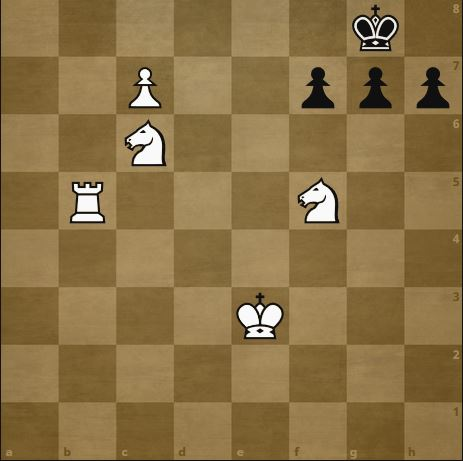
\includegraphics[width=0.5\textwidth]{random_position.jpg}
        \end{figure}
    \end{singlespace}

    Some possible moves for the white player would be: Nfe7+, Nce7+, Rb8\#, c8=Q\#, c8=B, Nxg7 or Kf3. Notice that to move a knight to e7, you must specify which knight moves there, as it is ambiguous. Using this knowledge we can move on to describing Portable Game Notation (PGN).

    Chess games nowadays are written down using PGN. The way PGN is formatted is by listing all of the moves played during a game using SAN, numbered by which turn it is, along with some added metadata like player names, dates, player ratings (ELO) and others. It is also all in ASCII, so it can be easily read by both humans and computer alike \cite{pgnrules}. Having this is a powerful tool as we can now simulate every single game in our dataset, as well as capturing metadata like player ratings, opening used, the date the game was played, the time control used and so on. From here, we can determine some way to convert this information into something more easily parsed by a neural network, as in changing everything into a numeric vector that can be passed into the network, as well as formatting what our output vector will have to look like.

    Now that we know we can model every possible move, we can move forward with modeling a board state using FEN. What FEN does is it encodes a board state using a single line of characters in the format: (board) (turn) (castling) (en-passant square) (halfmove clock) (fullmove number) \cite{pgnrules}. One example would be something like this: rnbqkbnr/pppppppp/8/8/4P3/8/PPPP1PPP/RNBQKBNR b KQkq e3 0 1 which is the board after the single move 1. e4 is played. Using this, we can model every possible board state including whether a pawn can be taken by en-passant or not, whether players have castling rights as well as half-move clocks for determining whether the game is a draw. This format can easily be converted into a vector of integers that can be passed into a neural network for training, especially if paired with an output vector of whether that board resulted in a win or loss for the white player. 

    \subsection{Search Trees}

    Seeing as we would like the create a chess engine, simply getting our neural network to predict whether a move is winning or not is not enough. Therefore, we must find some way for our approach to also generate possible move candidates and determine which is the most viable option for a win, using it's predictions. This means we will have to implement some sort of search tree algorithm. We can do it in the following way: modeling every possible move we can play, checking what the computer thinks is the best possible move and playing that one. 

    What we will be doing is implementing a version of alpha-beta search. What this does is it generates every possible move from a given position and gives each node a value, often based on some function determining a value for the resulting position \cite{alphabeta_montecarlo}. In our case, this will be the value our neural network generates when we pass positions into it. In our case, the white player will want to maximize the value and the black player will want to minimize it, in essence assuming best play from either player. 

    From here, in order to speed up our search, we can make an attempt at pruning branches. This is done by always keeping the current maximal value (called alpha) and the current minimal value (called beta). When you reach a node where the white player is making a move, whose value is less than the current alpha, there is no point in searching further down this branch, as it is already worse than what we currently consider to be the best move. The reverse is done for the black player with the beta value \cite{deepchess}\cite{alphabeta_montecarlo}. Using this will cut off some branches of the tree, effectively reducing the number of branches we need to check. We can set this up for a certain depth of search as well.

    What we will be doing is slightly different, but follows the same concept. We will be keeping alpha and beta as an entire board position, rather than a single value. Then when comparing, instead of using the neural network to grant a value to a position, we will instead pass into it two positions, from which it will decide the board state it considers to be better, from the white player's perspective \cite{deepchess}.
    
    \section{Our Model}

    \subsection{Inspiration}

    The primary inspiration for this work is that of the \href{http://dx.doi.org/10.1007/978-3-319-44781-0_11}{Deep Chess} paper. Essentially, we will be creating a Neural Network whose structure is heavily inspired by the one described in this paper. We also take some inspiration from \href{https://doi.org/10.1145/3394486.3403219}{Maia Chess} in terms of the goal of our project, as well as some from \href{https://github.com/LeelaChessZero/lc0}{Leela Chess Zero} and \href{https://arxiv.org/abs/1712.01815}{AlphaZero} in the fact that they are also Neural Networks designed to play chess, though their goals are slightly different. 

    What we will be doing is parsing the chess data from the lichess database, which contains many millions of games, filtering games and positions we do not want, converting positions into input vectors as well as an expected output for which board is considered better, from the white players perspective. When the network is trained, we can then create an alpha-beta search that will use our network to determine which branches of the tree to keep looking at and which ones to discard when considering different possible moves.

    \subsection{Parsing Chess Data}
    
    First thing we will have to do is parse the data from the lichess database in order to extract what we want from it. Seeing as our dataset is incredibly expansive and ranges from beginner players, to Grandmaster level players from time controls as fast as one minute all the way up to slow games lasting over an hour, this means we're going to want to reduce the amount of variability in the data, especially since our network will only be taking in positions as inputs. Players playing at different time controls and different skill levels will heavily increase the variety of the data, which may make it hard for the algorithm to predict whether a position is favourable or not, especially as the other data will not be given to it. As such, we will be only considering specific board states, similarly to Deep Chess, along with some other data filtering which we have chosen to try and shrink our dataset, considering our lack of computational resources.

    Because of this, we have made some limits. We will be limiting our data to:
    \begin{enumerate}
        \item Only games which ended decisively, as in no drawn games will be taken into our dataset. 
        \item Only games where both players are rated at least 1200 points in the lichess ranking system.
        \item Only games where each player has a minimum of twenty minutes to make all of their moves, excluding time increment.
        \item Only games which lasted at least ten moves.
    \end{enumerate}

    We will also be picking our games at random from the lichess database. As it is partitioned by month, our program will select a random order for the months and start from the top, considering all of our conditions for what will be a valid game or not. When it finds a game that is valid, it will select a random move between move ten and the end of the game, play the game up to that point and store the resulting position as well as the result of the game and the player ratings. We do this until we reach ten thousand positions in which white won the game and ten thousand positions in which black won the game, for a total of twenty thousand games. This means that when we go to train our network, which will compare two different boards, one where white wins and one where black wins, we will have a total of $10^{4} * 10^{4} = 10^{8}$ or one hundred million different possibilities. This should be more than enough data to adequately train our network. 

    The above means our program will have to be able to parse through the PGN in the lichess database and convert it into an input vector. This input vector, we will define as sixty-nine different values, sixty four for the different tiles of the board, four of them bits for castling rights and the last a bit for determining who's move it is. Each value for the board will contain a value between negative six and positive six, negative values for black pieces, positives values for white pieces and a zero for an empty tile. Although our autoencoder may suffer from the lack of total positions, we also lack the resources to recompute the PGN -> Input Vector computation every time we want to train, as well as the resources to merely store many hundreds of thousands, or even millions of board positions that we could generate from this database.
    
    We will be parsing the PGN and converting each move into a new board position, beginning with the starting position for chess, all the way up to the final move that we have randomly selected from the selected game. The resulting position will then be parsed and converted into the input vector as described above. Note that this is different than the input vector described in Deep Chess. They used a bit string 773 characters long as their input vector. This is called a bit-board representation \cite{deepchess}. We do not use this representation due to a lack of computational resources. A network that large would take a significantly larger amount of resources to train than we currently have access to.

    \subsection{Autoencoder}

    \begin{enumerate}
        \item Talk about what deepchess autoencoder looks like
        \item Talk about how we changed ours 
        \item Show how ours is structured, how we trained it and so on
    \end{enumerate}

    \subsection{Chess Network}

    \begin{enumerate}
        \item Talk about what deepchess looks like 
        \item Talk about how we changed ours 
        \item Talk about how ours is structured, how we trained it and so on
    \end{enumerate}

    \subsection{Playing Moves}

    \begin{enumerate}
        \item Talk about move tree 
        \item Talk about alphabeta
        \item Talk about deep chess' alpha beta 
        \item Talk about how we needed to use this as well 
    \end{enumerate}
    
    \section{Implementation}

    \subsection{Python-Chess}

    \begin{enumerate}
        \item Talk about the basics of the library
        \item Talk about why we used it (it's use)
        \item Parsing the lichess data
        \item Code snippets?
    \end{enumerate}

    \subsection{Tensorflow 2.0 and Keras}

    \begin{enumerate}
        \item Talk about the basics of tensorflow
        \item Talk about what keras is (high-level tensorflow)
        \item Talk about why we used keras (ease of use)
        \item Code snippets?
    \end{enumerate}

    \subsection{Different Alpha-Beta Search}

    \begin{enumerate}
        \item Talk about why we chose alpha-beta over monte carlo (we can choose depth of search easier)
        \item Talk about what we had to change about alphabeta
        \item Code snippets?
    \end{enumerate}
    
    \section{Conclusions}

    \subsection{Training Results}

    \begin{enumerate}
        \item Talk about autoencoder accuracy 
        \item Talk about deepchess accuracy 
        \item Talk about how awful the engine is 
        \item Code snippets?
    \end{enumerate}

    \subsection{Possible Problems}

    \begin{enumerate}
        \item Talk about ReLU for autoencoder (negative value issue)
        \item Talk about how we may have taken the wrong approach to training the autoencoder
        \item Talk about how maybe our network is a little small 
    \end{enumerate}

    \subsection{Possible Improvements}

    \begin{enumerate}
        \item Better quality data (higher rated players)
        \item Better filtering (excluding moves that were captures?)
        \item More input nodes (including en passant, player ratings etc)
        \item Different search method (monte-carlo)
        \item Whatever else we can think of
    \end{enumerate}

    \subsection{Future Possibilities}

    \begin{enumerate}
        \item With the improvements we can possibly create something that can play at different skill levels 
        \item Whatever else we can think of
    \end{enumerate}
    
    \clearpage
    \printbibliography

\end{document}